\chapter{The Standard Model and Beyond}
\label{ch:theory}
\epigraph{\emph{"Nothing in life is to be feared. It is only to be understood. Now is the time to understand more, so that we may fear less"}}{Marie Curie}


This thesis covers a search for new particles predicted by different scenarios beyond the \ac{SM}. In this chapter, the foundations for this search will be laid.
The chapter starts with a summary of the main concepts of the \ac{SM} used throughout this thesis in \Sect{\ref{sec:theory:sm}}. In said section, special focus is given on the Strong-force theory, on the hadron interactions in a \pp collision, and on the prompt-photon production process.
Then, a brief overview of the current limitations of the \ac{SM} is given in \Sect{\ref{sec:theory:bsm}}, to then present two different forms of New Physics that aim to solve the \ac{SM} shortcomings.
Finally, in \Sect{\ref{sec:theory:mc_simulation}}, the chapter ends with how these \ac{SM} processes are simulated using \ac{MC}, showing the different steps and tools to do so.




\section{The \acf{SM}}
\label{sec:theory:sm}

The \acf{SM} of particle physics is the mathematical theory that describes all the know elementary particles and their interactions.
The thoery has been developed through the ends of the 20\(^{\text{th}}\) century, being finalised by the md-1970s after the experimental confirmation of the quarks.
Over time, after many experiments backing its predictions, it has become the most complete and precise theory in particle physics. 

The \ac{SM} managed to describe, to present day, three of the four fundamental forces in nature: the \ac{EM}, the weak and the strong interactions.
These interactions work over different ranges and have different strenghts. Gravity, the fourth force, although not included in the \ac{SM}, is the weakest of the interactions and has an infinite range. The \ac{EM} interaction also has an infinite range but is much stronger than gravity. On the other hand, the weak and strong forces act on very short distances, and only dominate in the subatomic range. The weak interaction is weaker than the \ac{EM} and the strong, but still much stronger than gravity. Finally, the strong force is the strongest of them all.
The three forces described by the \ac{SM} arise from the exchange of mediator particles called \textit{bosons} between all matter particles, called \textit{fermions}.



\subsection{Elementary particles and their interactions}
\label{subsec:theory:sm:particles_interaction}

According to the \ac{SM}, all matter is made out of fermions, which are particles following the Fermi-Dirac statistics and have half-integer spin. These fermions interact between themselves by the exchange of the aforementioned bosons, which are particles of integer spin, following the Bose-Einstein statistics. Up to date, there has not been any single experiment capable of finding evidence that these fermions have internal structure.

\begin{figure}[ht!]
    \centering
    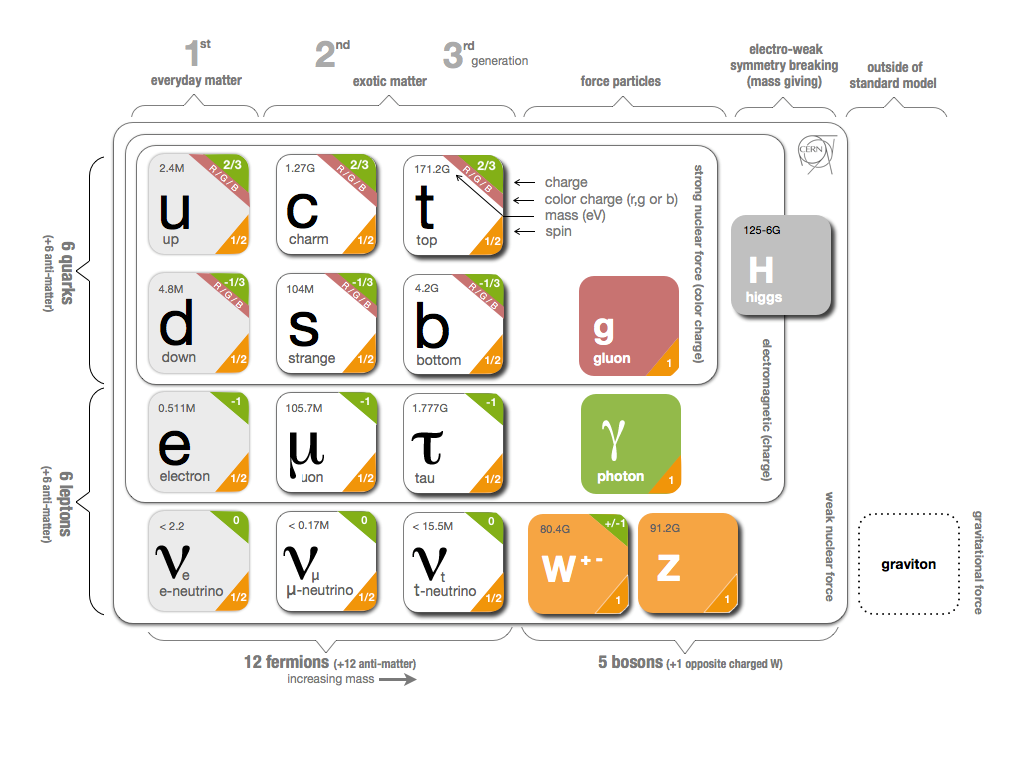
\includegraphics[width=\linewidth]{2_theory/sm}
    \caption{Overview of the particles of the \ac{SM}. All fermions participate in the weak interaction, but only the quarks interact with gluons, whereas both quarks and charged leptons interact with via the \ac{EM} force. Neutrinos, being neutral and colourless, only interact with the \Wboson and \Zboson bosons via the weak force. Finally, the graviton, although it has not been discovered yet, should be the corresponding force carrier of the gravity force. Extracted from \Refn{\cite{SM_diagram}}.}
    \label{fig:theory:sm:particles_interaction:particles}
\end{figure}

Fermions are divided into two kinds of elementary particles: leptons and quarks. There are six leptons classified according to their charge, and are divided into three families or generations, ordered based on their mass. Particles in higher generations have higher mass and are highly unstable, decaying into lower generation leptons. For this reason, matter is built on first generation leptons. The leptons are: electron (\(e\)), muon (\(\mu\)), and tau (\(\tau\)), with their respective neutrinos: electron neutrino (\(\nu_{e}\)), muon neutrino (\(\nu_{\mu}\)), and tau neutrino (\(\nu_{\tau}\)), and properties of each are shown in \Fig{\ref{fig:theory:sm:particles_interaction:particles}}.
There are also six antileptons, which have the opposite charge as the leptons, therefore increasing the number of leptons in the \ac{SM} up to 12. The electron, muon and tau, all have electric charge and sizable mass, while the neutrinos are electrically neutral and have very small mass.

Similarly, there are six flavours of quarks (also having their respective antiparticle): up (\(u\)), down (\(d\)), charm (\(c\)), strange (\(s\)), top (\(t\)), and bottom (\(b\)). Quarks also come in three different colours giving a total of 36 quarks, and only mix in such a way as to form colourless objects. An overview of the quarks and their properties are shown in \Fig{\ref{fig:theory:sm:particles_interaction:particles}}.


Each of the three forces unified in the \ac{SM} is described by a \ac{QFT}, corresponding to the exchange of a boson mediator.
The strong force, mediated by massless gluons, is responsible for binding quarks together. While gluons do not carry electric charge, they possess color charge, which leads to the phenomenon of \textit{color confinement}. Despite being massless, the strong interaction becomes stronger at low energies, confining quarks and gluons within hadrons due to the property asymptotic freedom and the aforementioned property of color confinement.
The \ac{EM} force is mediated between charged particles by photons. Photons do not have mass, and, as a consequence, the interaction has infinite range.
Finally, the weak interaction is mediated by the massive \Wboson and \Zboson bosons, leading to short-range interactions. The fundamental properties of these bosons are also displayed in \Fig{\ref{fig:theory:sm:particles_interaction:particles}}.









\subsection{Mathematical formulation of the \ac{SM}}
\label{subsec:theory:sm:mathematical}

The \ac{SM} is a renormalizable field theory based on local symmetries, providing a description of the fundamental particles and their interactions: the strong, the weak and the \ac{EM}. These interactions span by the requirement that the theory is invariant under local gauge transformations of the symmetry group:
\begin{equation*}
    SU(3)_{C} \times SU(2)_{L} \times U(1)_{Y},
\end{equation*}
where \(Y\) is the hypercharge, \(L\) the left-handed helicity and \(C\) the colour charge, and they represent the conserved quantities of the symmetry group. Every local gauge transformation can be absorbed within a gauge field, with the excitations of the gauge fields called gauge bosons. The \ac{EW} sector of the \ac{SM} \(SU(2)_{L} \times U(1)_{Y} \to U(1)_{\text{EM}}\) describes the weak and \ac{EM} interactions, after the spontaneous symmetry breaking mechanism by virtue of the Higgs potential. The non-abelian group \(SU(3)_C\) with colour charge desribes the strong interactions between quarks and gluons, and the theory is known as \ac{QCD}~\cite{Ellis-1996-book}.

In principle, the particles included in the \ac{SM} are massless, unlike the particles observed in nature. While the equations for the \ac{EW} interactions correctly describe particles like the photon, \Wboson, and \Zboson bosons, they fail to account for their masses. To address this, the concept of \ac{EWSB} was introduced, known as the Brout-Englert-Higgs mechanism~\cite{Higgs-1964_1,Higgs-1964_2,Higgs-1966,Englert_Brout-1964}. This mechanism explains how the \Wboson and \Zboson bosons acquire mass through the spontaneous breaking of the \ac{EW} symmetry, caused by the Higgs scalar field obtaining a non-zero vacuum expectation value. Furthermore, it predicts the existence of a new scalar particle, leading to a new massive boson with spin 0, called the Higgs bosons. This particle was experimentally confirmed in 2012 by the \ac{ATLAS} and \ac{CMS} collaborations at the \ac{LHC}, with a measured mass of \(125.25~\gev\)~\cite{ATLAS-HiggsObservation,CMS-HiggsObservation}.

The \ac{SM} Lagrangian can be separated into two terms: the first one describing the \ac{EW} interaction (\ac{EW} sector) and the second one representing the strong interactions (the strong sector):
\begin{equation*}
    \mathcal{L}_{\text{SM}} = \mathcal{L}_{\text{EW}} + \mathcal{L}_{\text{QCD}}
\end{equation*}








\subsubsection{The \acf{EW} interaction}


\subsubsection{The Higgs mechanism}


\subsubsection{\acf{QCD}}
\label{subsubsec:theory:sm:mathematical:qcd}

The huge effort to describe the rich spectrum of mesons and baryons resonances that were discovered during the 1950s, prompted Gell-Mann and Zweig to propose in 1964 the quark model~\cite{Gellmann-1964,Zweig-1964_1,Zweig-1964_2}, which asserts that hadrons are in fact composites of smaller constituents. Zweig called the elementary particles \textit{aces} while Gell-Mann called them \textit{quarks}, but finally the theory came to be called the quark model.

The quark model was formalised into the theory of \ac{QCD} with quarks carrying an additional quantum number called the colour charge, \(C=R,G,B\). Without colour charge, it would seem that the quarks inside some hadrons exist in symmetric quantum states, in violation of the Pauli exclusion principle.
The theory satisfies the gauge symmetry of the group \(SU(3)_C\), which has eight generators \(T^a = \frac{\lambda_{\alpha\beta}^a}{2}\), with \(\alpha\) and \(\beta\) being the color indices, \(\lambda_{\alpha\beta}^a\) the eight Gell-Man matrices (\(a=1,2,\dots,8\)). These eight generators introduce eight new phyisical gauge fields: the gluons.
Mesons and baryons, hadrons composed of two and three quarks respectively, are \textit{white} singles (neutral color charge) of \(SU(3)_C\). 

The local \(SU(3)_C\) symmetry is obtained by replacing in the lagrangian the covariant derivatives
\begin{equation*}
    D_{\mu} = \partial_{\mu} - i g_s \sum_{a=1}^{8} \frac{\lambda_{\alpha\beta}^a}{2} G_{\mu}^a,
\end{equation*}
where \(g_s\) is the bare \ac{QCD} coupling constant and is usually replaced by \(\alpha_s = g_s^2 / 4\pi\). The Yang-Mills field tensor \(G_{\mu\nu}^a\) for the group \(SU(3)_C\) can be written as
\begin{equation*}
    G_{\mu\nu}^a = \partial_{\mu} G_{\nu}^a - \partial_{\nu} G_{\mu}^a + g_s f_{abc} G_{\mu}^b G_{\nu}^c,
\end{equation*}
where \(f_{abc}\) are the structure constants of \(SU(3)\). It is important to note that the last term in the previous equation describes the gluon auto-interaction, responsible of the non-abelian nature of \ac{QCD}.
The \ac{QCD} Lagrangian density is then given by:
\begin{align*}
    \mathcal{L}_{\text{SM}} \supset \mathcal{L}_{\text{QCD}}
    &=
        -\frac{1}{2} \Tr\left\{G_{\mu\nu}G^{\mu\nu}\right\}
        + 
        \sum_{\text{flavours}} i \bar{q}_f \gamma^{\mu} D_{\mu} q_f\\
    &=
        -\frac{1}{4} \sum_{a=1}^{8} G_{\mu\nu}^a G^{\mu\nu}_a
        + 
        \sum_{\text{flavours}} i \bar{q}_f \gamma^{\mu} D_{\mu} q_f
\end{align*}

\paragraph{Renormalisation}

As mentioned, the \ac{SM} is a renormalisable \ac{QFT}. What this term refers to is briefly detailed in the following. Higher-order effects introduce quantum corrections, e.g., in the calculation of couplings in the \ac{SM}, which must be taken into account. At the same time, the particles in these loops have unbounded momenta, therefore divergences arise in the calculations for both low (\ac{IR}) and high (\ac{UV}) momenta, which must be eliminated for the theory to be consistent with experimental measurements. The process by which divergences disappear or are 'absorbed' by adding a scale dependence to parameters such as couplings or particle masses, is known as renormalisation. In this way the physical lagrangian, with couplings comparable to experiments, can be written as a bare lagrangian, minus a lagrangian containing the divergence-removing terms, at the cost of introducing a scale dependence \(\mu\) of the momentum. Therefore, the renormalisation results in the couplings (and other observables) being non-consistent and varying with \(\mu\). The phenomenom of asymptotic freedom and colour confinement in \ac{QCD} are consequences of this renormalisation process, which is in turn a property of gauge theories.

\paragraph{The running coupling constant \(\alpha_s\)}

One of the consequences of the non-abelian nature of \ac{QCD} appears on the renormalisation of the coupling constant \(\alpha_s\) via the vacuum polarisation diagrams, which ends up depending on the scale \(Q\) of interaction. For \ac{QED}, the vacuum polarisation is induced by virtual \ee pairs, which (shield) the electric charge and result in the coupling decreasing with distance. In contrast, gluons not only produce \qqbar-pairs (which cause an effect similar to \ac{QED}) but also create additional gluon pairs, which tend to anti-screen the apparent colour charge. In the high-energy regime (small distances), the coupling constant can be approximated with a 1-loop calculation in perturbative \ac{QCD}, as follows:
\begin{equation}
    \label{eq:theory:sm:mathematical:qcd:alphas}
    \alpha_s\left(Q^2\right) = 
    \frac{
        \alpha_s\left(Q^2_0\right)
    }{
        1 + \left(11 N_C - 2 N_f\right) \frac{\alpha_s\left(Q_0^2\right)}{12\pi} \log \left(\frac{Q^2}{Q_0^2}\right)
    }
    =
    \frac{
        12\pi
    }{
        \left(33 - 2 N_f\right)  \log \left(\frac{Q^2}{\Lambda_{\text{QCD}}^2}\right)
    },
\end{equation}
where \(N_C\) is the numbers of colors in the theory (3), \(N_f\) is the number of active flavours\footnote{Those quarks with \(m_q \ll Q\), where \(m_q\) is the quark mass after the process of \ac{EWSB} produced by the Higgs boson.}, \(\alpha_s\left(Q_0\right)\) is the value of the coupling constant at a fixed scale \(Q_0\), determined experimentally at the \Zboson mass value squared, and \(\Lambda_{\text{QCD}}\) is the cut-off \ac{IR} scale, where the perturbative approximation in \(\alpha_s\) stops being valid. Experimental measurements, compared to the theory prediction, of the running coupling constant \(\alpha_s\) is shown in \Fig{\ref{fig:theory:sm:mathematical:qcd:alphas}}, showing the excellent agreement between both.

\begin{figure}[ht!]
    \centering
    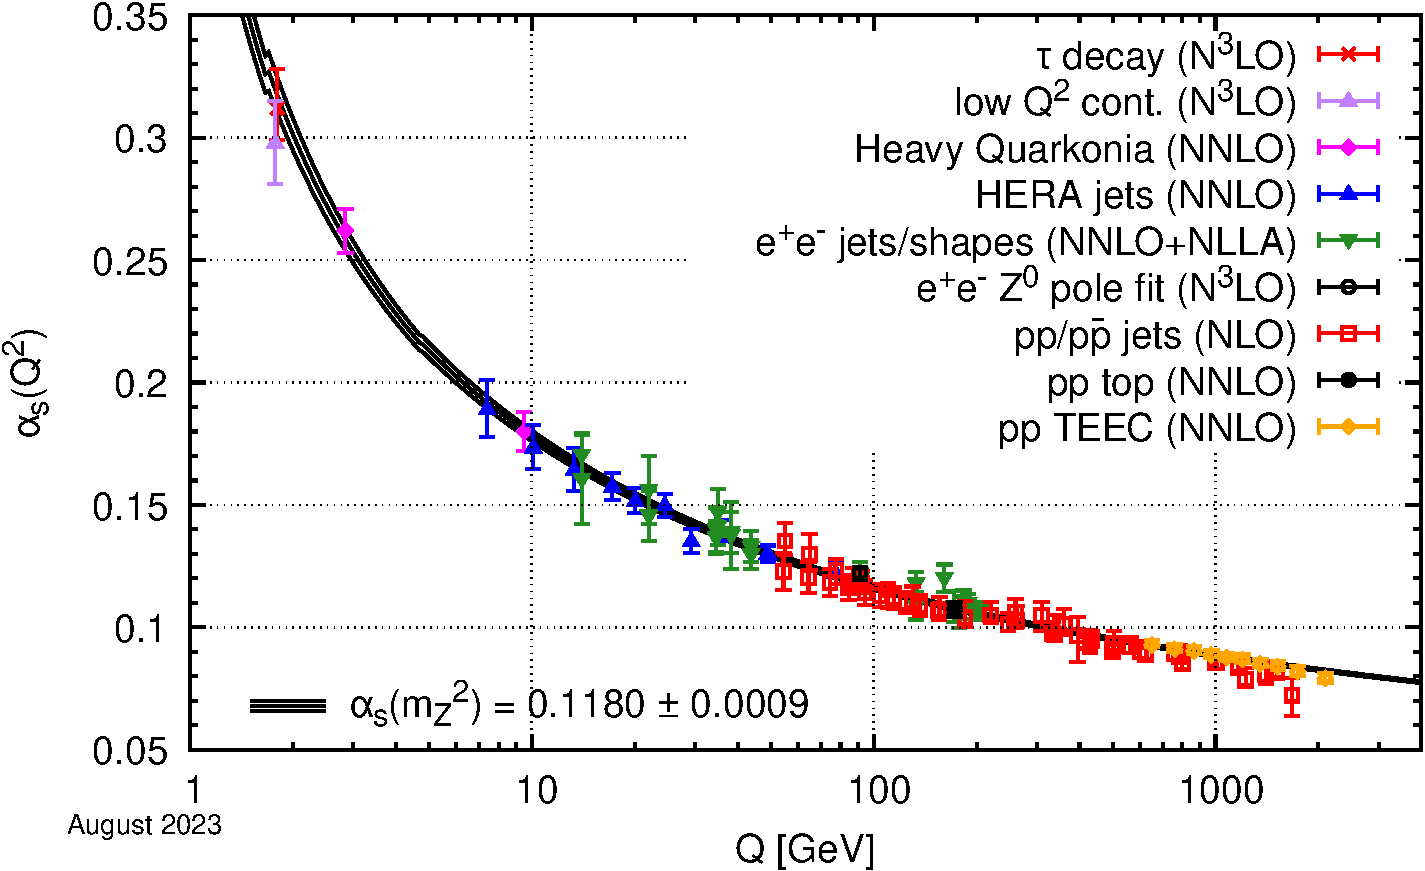
\includegraphics[width=0.6\linewidth]{2_theory/alphas}
    \caption{Experimental measurements of the coupling constant of \ac{QCD} compared to the coupling computed at five loops~\cite{ParticleDataGroup2024}.}
    \label{fig:theory:sm:mathematical:qcd:alphas}
\end{figure}


\paragraph{Asymptotic freedom and confinement}

The coupling constant is said to run, being large at low energy and becoming smaller at high energy. From \Eqn{\ref{eq:theory:sm:mathematical:qcd:alphas}}, at high energies \(\alpha_s \to 0\) therefore \ac{QCD} interacts weakly, allowing the quarks as unbounded particles, phenomenom known as asymptotic freedom~\cite{Wilczek_Gross-1973,Politzer-1973}.
On the other hand, for low energies (\(Q^2 \to 0\)), the coupling \(\alpha_s\) increases divergently, and therefore \ac{QCD} is strongly interacting leading to the confinement of quarks and gluons~\cite{Glashow_Georgi-1974}. Confinement implies that neither quarks nor gluons can appear in isolation, they can only exist within colourless composite "partons", called hadrons.
Moreover, starting from the infrared cut-off scale \(\Lambda_{\text{QCD}}\), where perturbative approximation at \(\alpha_s\) is no longer valid, the creation of quark-antiquark pairs in the vacuum is more energetically favourable than the separation of a pair of bound quarks. For this reason, as they lose energy, the quarks and gluons produced in a proton collider undergo a repetitive process known as hadronisation, in which collimated cascades of hadrons, called jets, are created, forming a cone from the initial quark or gluon to the calorimeters, where all their energy is deposited.


\subsection{Hadron interactions in \pp colliders}
\label{subsec:theory:sm:hadron_interactions}

As discussed in \Sect{\ref{subsubsec:theory:sm:mathematical:qcd}}, the coupling constant \(\alpha_s\), which governs the strong interactions between quarks, has a strong dependence on the energy scale of each interaction, radically modifying the nature of the processes. The modelling of a proton-proton collision in an experiment like \ac{ATLAS}, where it is necessary to know its evolution from the interaction between the protons at \(\sqs \sim \tev\), to the interaction of the particles in the final state with the active and passive materials of the detector at a few GeV, represents a huge challenge, as it covers very different behaving \ac{QCD} regimes. Given that the \ac{LHC} is a proton collider, it is mandatory to have a very precise description of the proton structure, as a \pp collision at very high energies is basically to collide the constituents of them.

At very high energies, but within the perturbative regime, the collision between two protons can be studied via the Parton Model. This model has been introduced by Feynman~\cite{Feynman-1969} and Bjorken~\cite{Bjorken-1969_1} in the late-1960s, to interpret electron-nucleon deep inelastic scattering at SLAC. This description has proven to be a good approximation for parton-parton interactions with large momentum transfer (i.e. Bjorken scaling~\cite{Bjorken-1969_2}) but is not appropriate for modelling the interaction at low energies.
Under this abstraction, the partons include not only the valence quarks (\(u\), \(\bar{u}\) and \(d\) in the case of the proton), but also the pairs of particles and antiparticles in the quark sea, and the gluons that mediate the interactions between them. The model assumes a permanent interaction between partons, so their individual momentum is unknown, although their fraction of momentum with respect to the total hadron momentum can be modelled as a random variable.
Furthermore, in the case of experimental verification, the quarks and gluons in the final state are not directly observed due to hadronisation (concept discussed in \Sect{\ref{subsec:theory:mc_simulation:hadronisation}}). Instead, an effective hadronic cross section, \(\sigma(\pp\to jj)\), is calculated between the incident protons and the final state jets. To perform this passage, the factorisation theorem~\cite{Ellis_Georgi_Politzer_Ross-1978,Feynman-1969,Collins_Soper_Sterman-book,Collins_Soper-1987} is used, which allows a systematic separation between the short-distance interactions (of the partons), and the long-distance interactions (responsible for colour confinement and hadron formation). This theorem states that the total cross-section for two hadrons can be obtained by weighting and combining the cross-sections for two particular partons. This weighting is done using \(f_i(x,Q^2)\), the \acp{PDF1}, which describe the parton density for a parton of species \(i\) in a hadron, with a fraction \(x\) of the hadron energy-momentum when the hadron is probed at a resolution scale \(Q^2\). The cross-section for a hard scattering process \(\pp \to X\), initiated by two hadrons with four-momenta \(P_1\) and \(P_2\) can be written as:
\begin{equation}
    \label{eq:theory:sm:hadron_interactions:xs}
    \sigma_{\pp\to X} = \sum_{ij} \int_0^1 \dd{x_1} \dd{x_2} f_i(x_1, \mu_F^2) f_j(x_2, \mu_F^2) \, \hat{\sigma}_{ij}\left(p_1, p_2, \alpha_s(\mu_R^2), Q^2/\mu_R^2, Q^2/\mu_F^2 \right),
\end{equation}
where \(x_1\) and \(x_2\) are the momentum fractions carried by the interacting partons, and \(p_1 = x_1 P_1\) and \(p_2 = x_2 P_2\) are the interacting parton momenta. The partonic cross-section \(\hat{\sigma}_{ij}\), corresponding to the interaction of partons \(i\) and \(j\), is calculated at a fixed order in \(\alpha_s\), which is evaluated at some renormalisation scale, \(\mu_R\) and factorisation scale \(\mu_F\). The renormalisation scale \(\mu_R\) is important to absorb \ac{UV} divergences in calculations at higher orders. The total cross-section is obtained by summing over all possible parton flavours and integrating over all possible momentum fractions. The parton distribution functions, \(f_i\) and \(f_j\), are evaluated at a factorisation scale, \(\mu_F\) , which can be thought of as the scale that separates short-distance, perturbative physics, from long-distance, non-perturbative physics (i.e., separates hard and soft processes).

If the perturbative expansion were carried to all orders, the cross-section in \Eqn{\ref{eq:theory:sm:hadron_interactions:xs}} would be independent of \(\mu_F\) and \(\mu_R\). However, in actual finite order calculation this does not hold. They are usually both taken to be equal, \(\mu_F = \mu_R = \mu\), chosen at the typical scale \(Q^2\) of the process, in order to minise the contribution of uncalculated higher order terms, whose forms are logarithmic \(\log\left(Q^2/\mu_R^2\right)\) and \(\log\left(Q^2/\mu_F^2\right)\). The dependence of the prediction on \(\mu_R\) and \(\mu_F\) is assigned as a theoretical uncertainty. The fact that the cross-section of a process should be independent of the factorisation scale \(\mu_F\) led to the DGLAP equations (Dokshitzer-Gribov-Lipatov-Altarelli-Parisi)~\cite{Dokshitzer-1977,Gribov_Lipatov-1971,Altarelli_Parisi-1977}. These equations determine the evolution of the \ac{PDF1} with \(Q^2\).
For the case of the proton, \Fig{\ref{fig:theory:sm:hadron_interactions:pdfs}} shows the \acp{PDF1} evaluated at two different factorisation scales for all possible partons.

\begin{figure}[ht!]
    \centering
    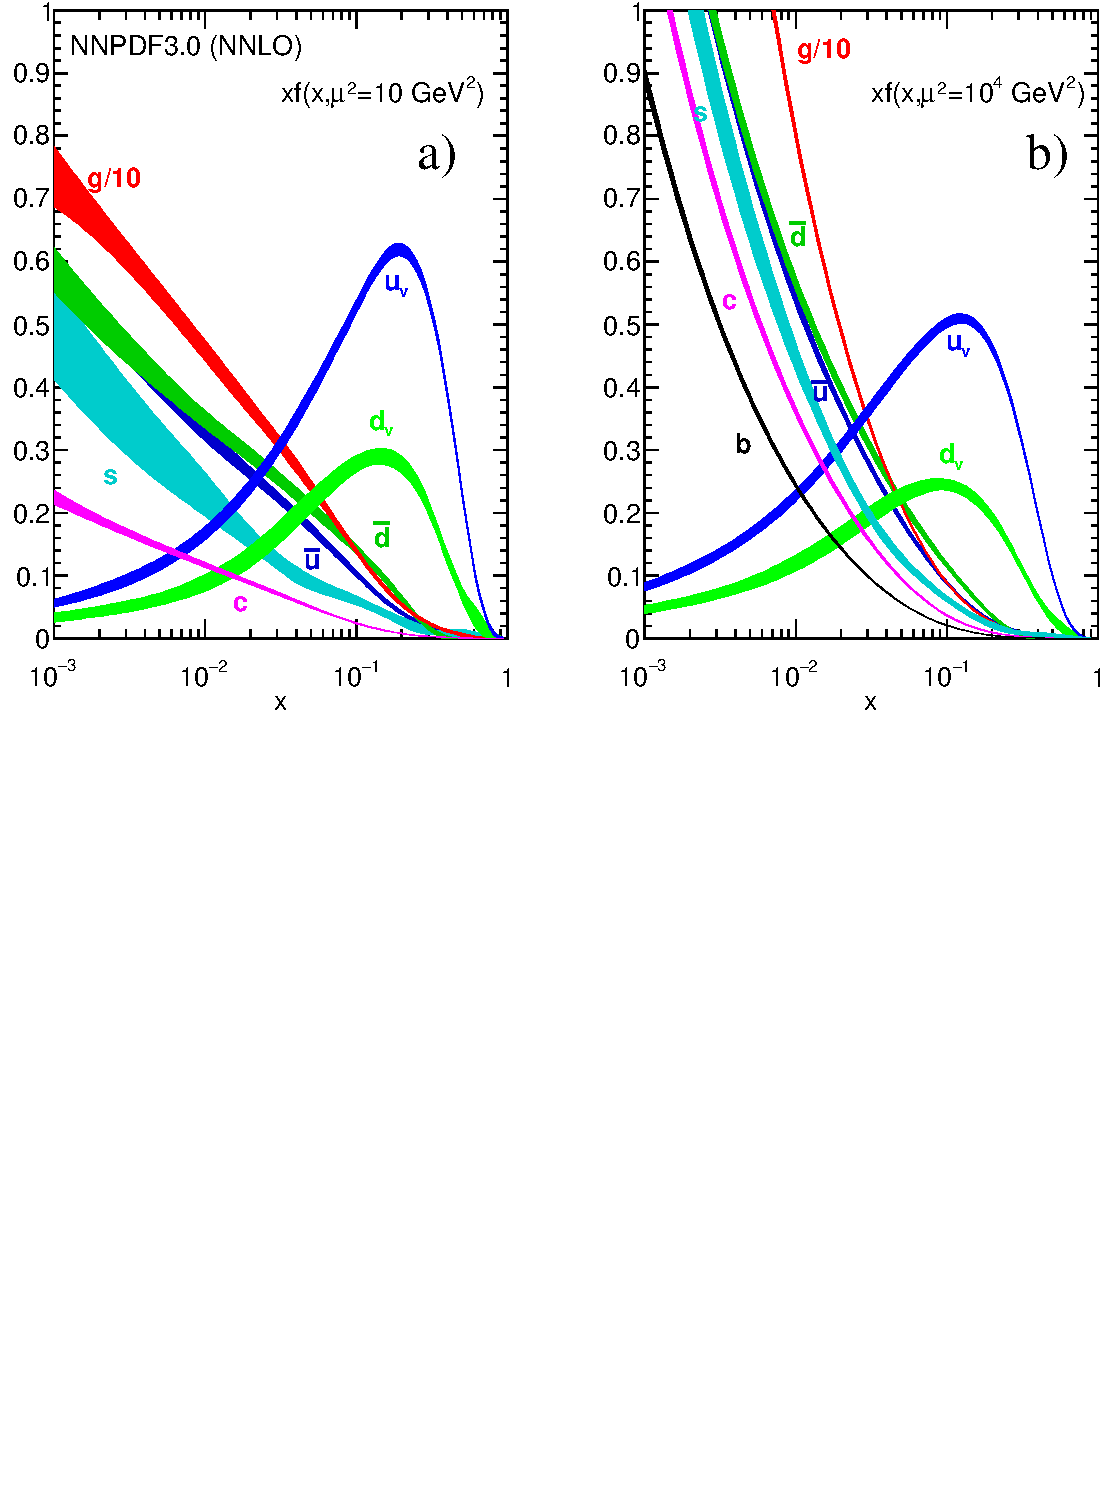
\includegraphics[width=0.7\linewidth]{2_theory/pdfs}
    \caption{Parton momentum fraction \(x\) times the unpolarized parton distributions \(f_i(x, Q^2)\) (where \(i = u_v = u - \bar{u}, \, d_v = d - \bar{d},\, \bar{u},\, \bar{d},\, s\simeq\bar{s},\, c=\bar{c},\, b=\bar{b},\, g \)) obtained in the NNLO NNPDF3.0 global analysis~\cite{NNPDF} at scales \(\mu^2 = 10~\gev^2\) (left) and \(\mu^2 = 10^4~\gev^2\) (right) with \(\alpha_s(M_Z^2) = 0.118\). Figures extracted from \Refn{\cite{ParticleDataGroup2020}}.}
    \label{fig:theory:sm:hadron_interactions:pdfs}
\end{figure}




\subsubsection{Process description}

Initially two hadrons are coming in on a collision course, where each hadron can be thought as a group of essentially collinear partons quantitatively characterised by the parton distributions. In a collision scenario with accelerated particles carrying \ac{EM} and colour charges, bremsstrahlung can occur, e.g. as gluon radiation such as \(q \to qg\). A collision between two partons, one from each side, takes place producing the hard process of interest, that can be calculated by a perturbative approach to some order in \(\alpha_s\), which corresponds to the number of outgoing partons. Emissions that are started off from the two incoming colliding partons are called \ac{ISR}, while radiations from the outgoing partons are referred as \ac{FSR}. With the parton shower development, the colour field strength increases as partons loose energy and they can break up by the production of quark-antiquark pairs. Thus, quarks and antiquarks may combine to produce a primary hadron. The creation of hadrons as a consequence of the confinement phenomenon is referred to as “hadronisation”. The additional products of the collision that are not explicitely related to the hard process (radiation, hadron remnants, products of multiple parton interactions, etc.), are generally grouped altogether and called \ac{UE}. A visualisation of the \pp collision is shown in \Fig{\ref{fig:theory:sm:hadron_interactions:parton_shower}}.



\begin{figure}[ht!]
    \centering
    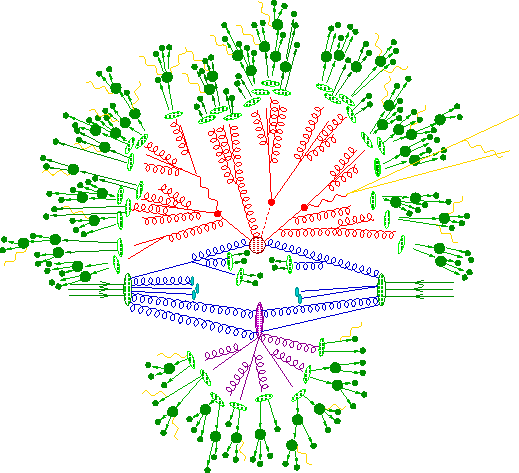
\includegraphics[width=0.7\linewidth]{2_theory/parton_shower}
    \caption{Illustration of the stages of a hadron-hadron collision. The red circle in the center of the figure represents the hard collision, surrounded by a tree-like structure representing bremmstrahlung radiation as simulated by parton showers. The purple blob at the botton represents the \ac{UE}. The hadronisation process is represented by the light green blobs, dark green blobs indicate hadron decays, while yellow lines signal soft photon radiation~\cite{Hoche-2015}.}
    \label{fig:theory:sm:hadron_interactions:parton_shower}
\end{figure}



Over the years, different \ac{LHC} experiments have measured cross sections of different \ac{SM} processes. \Fig{\ref{fig:theory:sm:hadron_interactions:sm_results}} shows the good agreement between the \ac{ATLAS}-measured cross sections of some processes and their theoretical predictions.


\begin{figure}[ht!]
    \centering
    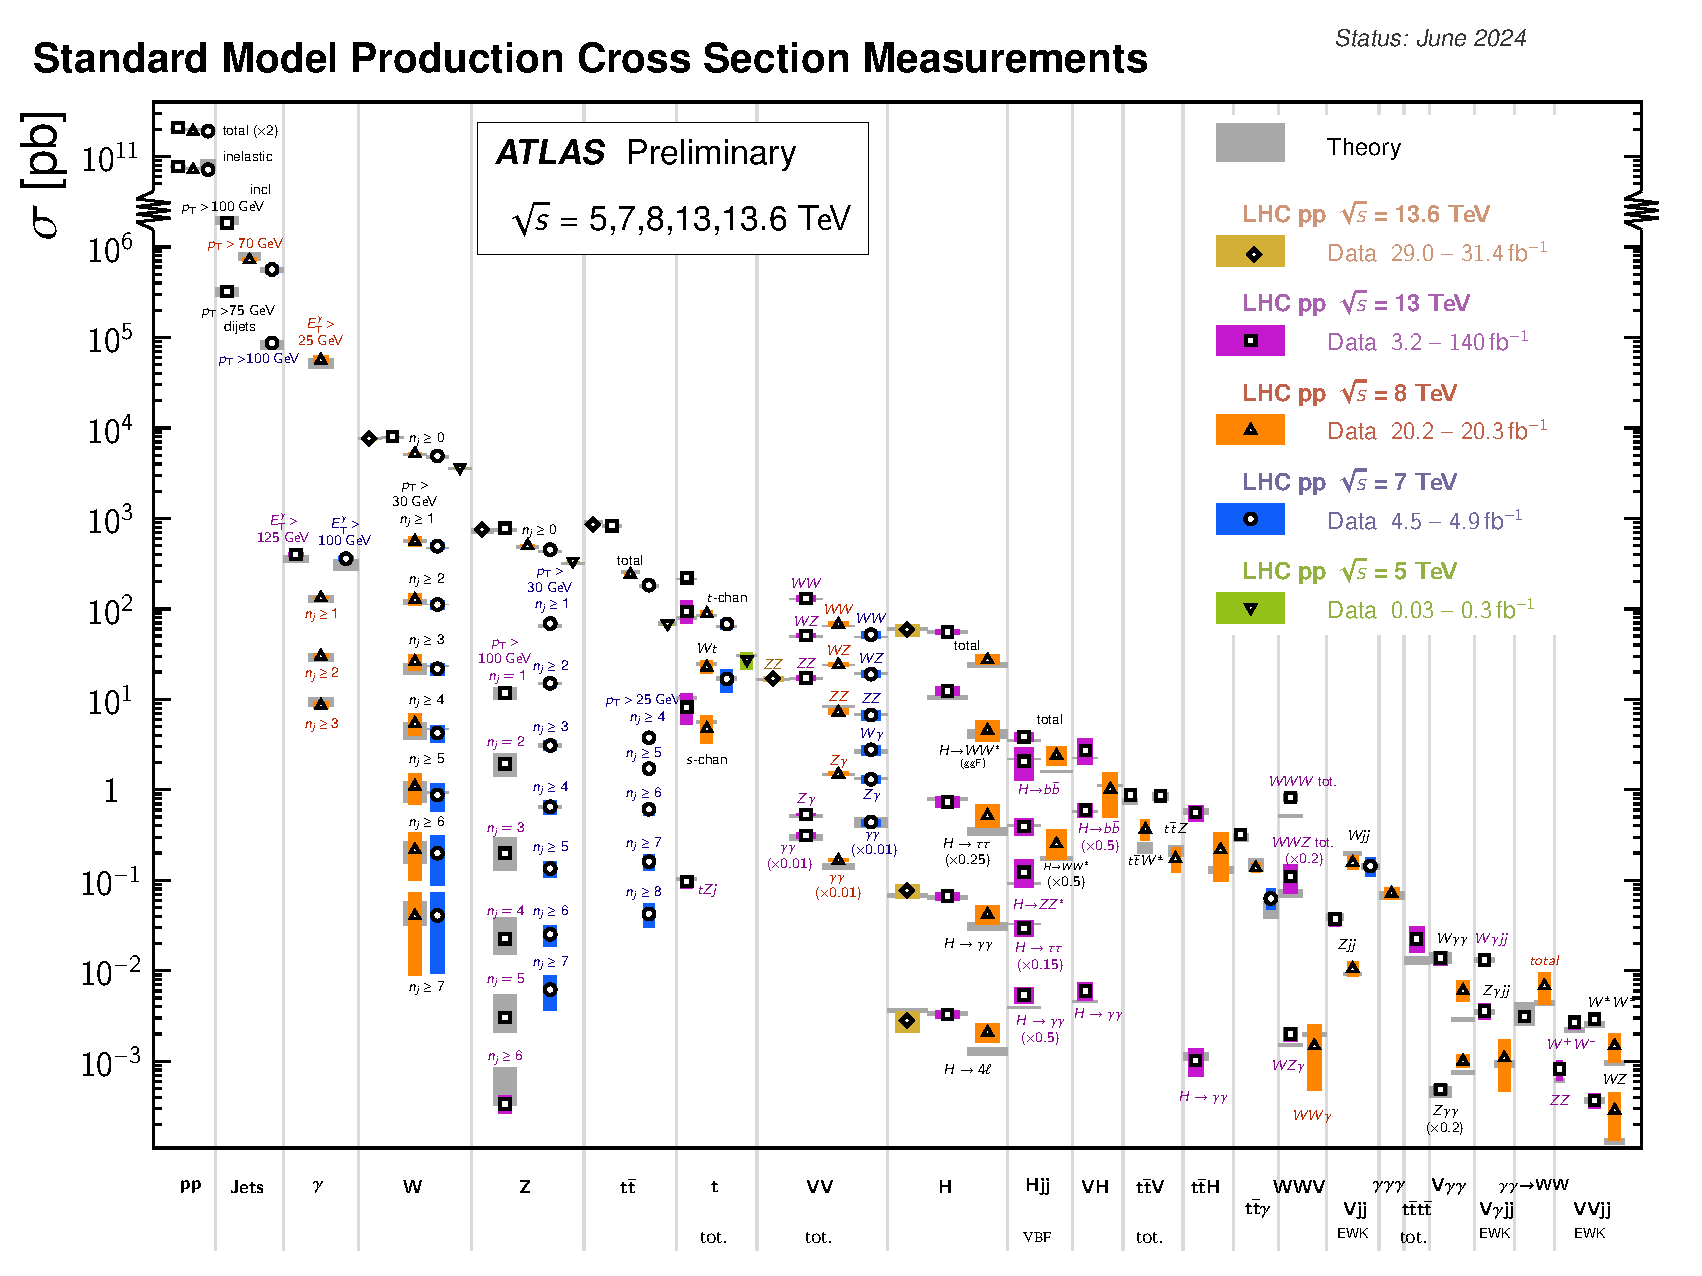
\includegraphics[width=0.8\linewidth]{2_theory/sm_measurements}
    \caption{Summary of several Standard Model total and fiducial production cross-section measurements, compared against their theoretical predictions~\cite{ATLAS-SM_Measurements}.}
    \label{fig:theory:sm:hadron_interactions:sm_results}
\end{figure}



\subsection{Theory of prompt-photon production}
\label{subsec:theory:sm:prompt_photon}


High transverse momentum ("prompt") photons constitute colourless probes of the hard interaction and their  production in proton-proton collisions, \(\pp \to \gamma+X\), provides a testing ground for QCD, whose measurement offers certain advantages over other analyses in jet production events, the most abundant process in single hadron colliders. In this case, the presence of a \ac{QED} vertex at \ac{LO} makes the theoretical calculations more reliable and gives access to a lower range of \pt. Moreover, the energy resolution of electromagnetic calorimeters are in general better than those of the hadronic calorimeter\footnote{A description of both calorimeters is given in \Ch{\ref{ch:atlas}}.}, and systematic uncertainties in the photon energy scale are smaller. Due to the fact that photons do not hadronise (see \Sect{\ref{subsec:theory:mc_simulation:hadronisation}}), the direction and energy of photons is straightforwardly measured in the calorimeter without the need for a jet algorithm to reconstruct a jet.

Prompt-photon production proceeds via two processes: the direct-photon process (D), in which the photon arises directly from the hard interaction, and the fragmentation-photon process (F), in which the photon is emitted in the fragmentation of a high transverse momentum parton~\cite{Szczurek_Pietrycki-2007,Belghobsi_Fontannaz-2009}. From a topological point of view, when a direct photon is produced, it is most likely that it will be separated from the hadronic activity, whereas a photon produced from a fragmentation process, is most probably accompanied by hadrons.

At \ac{LO} in perturbation theory, there are two subprocesses that contribute to the direct-photon production: (a) the Compton process \(qg \to \gamma q\), and (b) the annihilation process \(\qqbar \to \gamma+g\), shown in \Figs{\ref{fig:theory:sm:prompt_photon:feynman_lo_direct:compton}}{\ref{fig:theory:sm:prompt_photon:feynman_lo_direct:annihilation}}. At medium and large \(x\), there is a natural hierarchy of parton distributions in the proton, \(q \gg g \gg \bar{q}\), while at small \(x\), \(g \gg q,\bar{q}\). As a consequence, in proton-proton collisions, the \(qg\) Compton process dominates over essentially all the \pt range. This makes direct photon production particularly useful for constraining the gluon distribution.

\begin{figure}[ht!]
    \centering
    \begin{subfigure}[h]{0.49\linewidth}
        \centering
        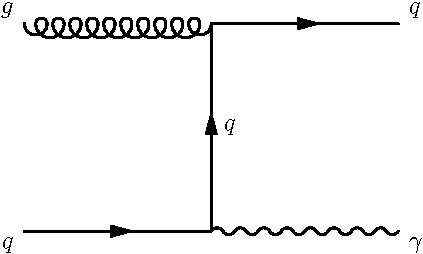
\includegraphics[width=0.7\linewidth]{2_theory/diagrams/gammajet_compton}
        \caption{Compton.}
        \label{fig:theory:sm:prompt_photon:feynman_lo_direct:compton}
    \end{subfigure}
    \hfill
    \begin{subfigure}[h]{0.49\linewidth}
        \centering
        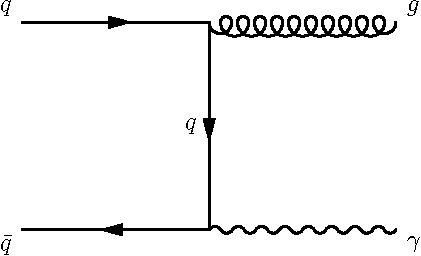
\includegraphics[width=0.7\linewidth]{2_theory/diagrams/gammajet_annihilation}
        \caption{annihilation.}
        \label{fig:theory:sm:prompt_photon:feynman_lo_direct:annihilation}
    \end{subfigure}
    \caption{Feynman diagrams for the \ac{LO} direct-photon production in \pp collisions.}
    \label{fig:theory:sm:prompt_photon:feynman_lo_direct}
\end{figure}

\ac{NLO} corrections to this process are represented in \Fig{\ref{fig:theory:sm:prompt_photon:feynman_nlo_direct}}. In \Fig{\ref{fig:theory:sm:prompt_photon:feynman_nlo_direct:gluon}}, there is a collinear singularity when the momenta of the final-state quark and gluon are parallel. This divergence cancels when real and virtual gluon contributions (see \Fig{\ref{fig:theory:sm:prompt_photon:feynman_nlo_direct:gluon_virtual}}) are summed, and the net effect is a finite \(\mathcal{O}(\alpha_s)\) correction to the \ac{LO} process. On the other hand, in the diagram of \Fig{\ref{fig:theory:sm:prompt_photon:feynman_nlo_direct:photon}} there is another collinear singularity, this time, when the photon and quark momenta are parallel. This singularity, however, does not cancel, but has to be absorbed into a photon fragmentation function \(D_q^{\gamma} (z, \mu^2_f )\) that represents the probability of finding a photon carrying longitudinal momentum fraction \(z\) in a quark jet at scale \(\mu_f\). This fragmentation function is not calculable in perturbation theory, and obeys a DGLAP evolution equation similar to that for the hadron fragmentation functions. The contribution to the cross section from \Fig{\ref{fig:theory:sm:prompt_photon:feynman_nlo_direct:photon}} contains a piece of the form
\begin{equation}
    \label{eq:theory:sm:prompt_photon:fragmentation_contribution}
    \hat{\sigma}(qg \to qg) \oplus D_q^{\gamma} \left(z, \mu_f^2\right).
\end{equation}
The photon-fragmentation contribution appears when a final-state quark-photon collinear singularity occurs in the calculation of the contribution from subprocesses such as \(qg \to gq\gamma\). At higher orders, multiple final-state collinear singularities appear in any subprocess where a high-\pt parton undergoes a cascade of successive collinear splittings ending up with a quark-photon splitting. These singularities are factorised to all orders in \(\alpha_s\) according to the factorisation theorem, and are absorbed into quark and gluon fragmentation functions of the photon, \(D_q^{\gamma} \left(z, \mu_f^2\right)\) and \(D_g^{\gamma} \left(z, \mu_f^2\right)\), respectively.

\begin{figure}[ht!]
    \centering
    \begin{subfigure}[h]{0.32\linewidth}
        \centering
        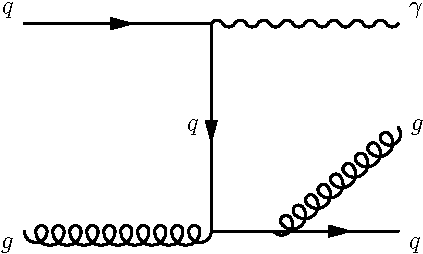
\includegraphics[width=\linewidth]{2_theory/diagrams/gammajet_fsr_gluon}
        \caption{Gluon \ac{FSR}.}
        \label{fig:theory:sm:prompt_photon:feynman_nlo_direct:gluon}
    \end{subfigure}
    \hfill
    \begin{subfigure}[h]{0.32\linewidth}
        \centering
        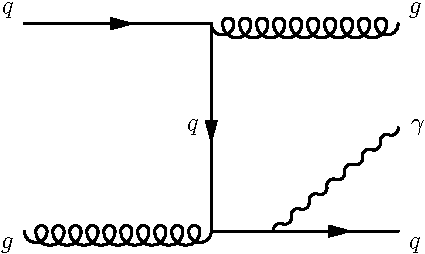
\includegraphics[width=\linewidth]{2_theory/diagrams/gammajet_fsr}
        \caption{Photon \ac{FSR}.}
        \label{fig:theory:sm:prompt_photon:feynman_nlo_direct:photon}
    \end{subfigure}
    \hfill
    \begin{subfigure}[h]{0.32\linewidth}
        \centering
        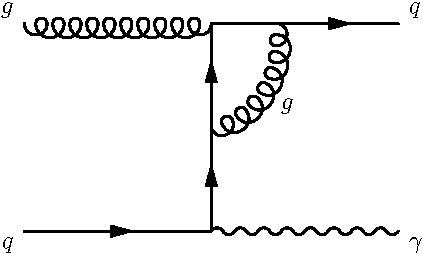
\includegraphics[width=\linewidth]{2_theory/diagrams/gammajet_nlo_direct_virtualcorrection}
        \caption{Virtual gluon correction.}
        \label{fig:theory:sm:prompt_photon:feynman_nlo_direct:gluon_virtual}
    \end{subfigure}\\
    \caption{Feynman diagrams for direct-photon production at \ac{NLO} in \pp collisions.}
    \label{fig:theory:sm:prompt_photon:feynman_nlo_direct}
\end{figure}


The photon fragmentation function increases uniformly with the scale over the whole \(z\) range, i.e. \(D_k^{\gamma} \left(z, \mu_f^2\right) \sim d^{\gamma}(z)\ln(\mu^2)\) as \(\mu^2 \to \infty\). When the \pt is large with respect to \(\sim 1~\GeV\), the \(\ln \pt^2\) growth of the fragmentation function in \Eqn{\ref{eq:theory:sm:prompt_photon:fragmentation_contribution}} compensates one of the \(\alpha_s \left(\pt^2\right)\) couplings in the subprocess cross section, and the contribution is effectively of order \(\alpha_s \left(\pt^2\right) \alpha_{EM}\), i.e. the same as the \ac{LO} contribution. Feynman diagrams corresponding to the \ac{LO} fragmentation component are shown in \Fig{\ref{fig:theory:sm:prompt_photon:feynman_lo_frag}}.



\begin{figure}[ht!]
    \centering
    \begin{subfigure}[h]{0.49\linewidth}
        \centering
        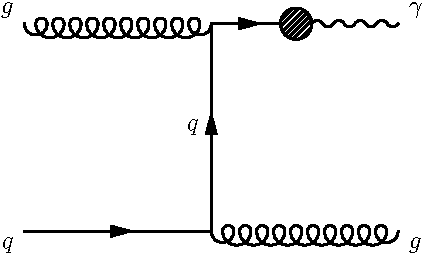
\includegraphics[width=0.7\linewidth]{2_theory/diagrams/gammajet_fragmentation_quark}
        \caption{\ac{NLO} quark fragmentation.}
        \label{fig:theory:sm:prompt_photon:feynman_lo_frag:quark}
    \end{subfigure}
    \hfill
    \begin{subfigure}[h]{0.49\linewidth}
        \centering
        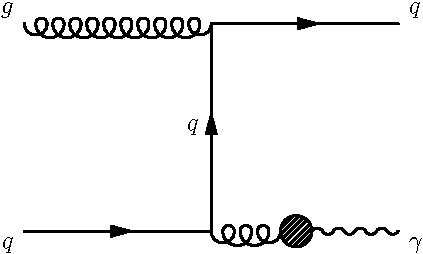
\includegraphics[width=0.7\linewidth]{2_theory/diagrams/gammajet_fragmentation_gluon}
        \caption{\ac{NLO} gluon fragmentation.}
        \label{fig:theory:sm:prompt_photon:feynman_lo_frag:gluon}
    \end{subfigure}\\
    \caption{Feynman diagrams for the \ac{LO} fragmentation-photon processes in \pp collisions (\subref{fig:theory:sm:prompt_photon:feynman_lo_frag:quark}) \(qg \to g q(\gamma)\) and (\subref{fig:theory:sm:prompt_photon:feynman_lo_frag:gluon}) \(qg \to q g(\gamma)\).}
    \label{fig:theory:sm:prompt_photon:feynman_lo_frag}
\end{figure}


The inclusive differential cross section in \(\etgam\) for the production of a non-isolated photon is given by the sum of the direct and fragmentation contributions

\begin{align}
    \dv{\sigma}{\etgam} &= \dv{\sigma_{\text{dir}}}{\etgam} + \dv{\sigma_{\text{frag}}}{\etgam} \nonumber\\
    &= \sum_{a,b=q,\bar{q},g} \int \dd{x_a} \dd{x_b} f_a\left(x_a, \mu_F^2\right) f_b\left(x_b, \mu_F^2\right) \times \nonumber\\
    &\quad
    \left[
        \dd{\hat{\sigma}^{\gamma}_{ab} \left(p^{\gamma}; x_a, x_b, \mu_R, \mu_F, \mu_f\right)}
        +
        \sum_{c=q,\bar{q}, g} \int_{z_{\min}}^{1} \frac{\dd{z}}{z^2} \dd{\hat{\sigma}^c_{ab} \left(p^{\gamma}; x_a, x_b, z, \mu_R, \mu_F, \mu_f\right)} D_c^{\gamma} \left(z, \mu_f^2\right)
    \right]
\end{align}


where \(D_c^{\gamma} \left(z,\mu_f^2\right)\) is the fragmentation function of a parton \(c\) to a photon carrying momentum fraction \(z\), \(f_a \left(x_a, \mu^2_F \right)\) is the \ac{PDF1} of a parton \(a\), \(\mu_R\) and \(\mu_F\) are the standard renormalisation and factorisation scales, and \(\mu_f\) is the fragmentation scale. Corrections to the direct component of the partonic cross section \(\hat{\sigma}^{\gamma}_{ab}\) are known up to the \ac{NNLO} in \ac{pQCD}, while the fragmentation component \(\hat{\sigma}^c_{ab}\) is only known at \ac{NLO}.

At \ac{LO}, the theory calculations for the direct and fragmentation processes converge separately, and can be considered independently. However, this distinction has no physical meaning beyond the \ac{LO}, since both kinds of processes need to be considered at the same time to cancel the final-state infrared and collinear singularities. Therefore, beyond the \ac{LO}, both direct and fragmentation processes cannot be considered separately. From a theoretical point of view, the distinction is defined by an arbitrary choice. It follows from the necessity of factorising the final-state collinear singularities and absorbing them into the fragmentation functions. This factorisation requires the introduction of an arbitrary fragmentation scale \(\mu_f\) , which is a non-physical parameter. More generally, it relies on the arbitrary choice of the factorisation scheme, which defines the finite part of the higher-order corrections that is absorbed in the fragmentation functions together with the singularities; the remaining finite part is then included in the higher-order contributions to the partonic cross sections. The dependence on this arbitrariness, and in particular, on \(\mu_f\), cancels only in the sum of the direct and fragmentation contributions, so only this sum is a physical observable.






\section{Physics \acf{BSM}}
\label{sec:theory:bsm}

The previous section briefly described most of the properties of the \ac{SM}, together with \ac{ATLAS} results showing how well the \ac{SM} agrees with experimental data. Despite being one of the most successful theories in physics in general, the model naturally has a range of validity.
However, it cannot be considered the final theory (the one that could "explain everything"), as it has certain limitations, both from a theoretical and an experiential point of view. The \ac{SM} is still regarded as an effective theory, a low-energy approximation of a more fundamental theory. There are three popular types of new physics theories: (i) models with an extended (family) symmetry or scalar sector, (ii) higher dimensional theory, and (iii) quark-lepton compositeness (namely, the \ac{SM} fermions are not elementary anymore~\cite{Kuhn_Zherwas-1984,Cabibbo_Maiani_Srivastava-1984,DeRújula_Maiani_Petronzio-1984,Baur_Spira_Zerwas-1990,Bhattacharya_Chauhan_Choudhary_Choudhury-2009,Zhan_Li_Liu_Li-2016}).
In the following, a general overview of the main shortcomings of the \ac{SM} are presented. After that, the two last types of new physics theories are discussed, enumerating the theoretical models used in the search carried out in this thesis.

\begin{itemize}
    \item \underline{Gravity:} One of the main limitations of the \ac{SM} is the impossibility of including gravity in the same way as other interactions. Not only is including gravity in the theory not enough to explain the observations, but the mathematics used in the \ac{SM} is practically incompatible with the formulation of General Relativity.
    \item \underline{Hierarchy Problem:} In the context of high energy physics, a hierarchy problem occurs when the fundamental value of some physical parameter (such as a coupling constant or a mass), in some Lagrangian is vastly different from its effective value, which is the value that gets measured in an experiment. Typically the renormalised value of parameters are close to their fundamental values, but in some cases, it appears that there has been a delicate cancellation between the fundamental quantity and the quantum corrections. In general, hierarchy problems are related to fine-tuning of the parameters in the theory. The most well-known case in particle physics is the difference on the \ac{EW} scale \(M_W \sim 10^2~\gev\) and Planck scale, where quantum gravity effects start to take over \(M_P\sim10^{19}~\gev\), whose ratio is \(M_W / M_P \sim 10^{-17}\).
    \item \underline{\acf{DM}:} A hint towards the incompleteness of the \ac{SM} is the presence of \ac{DM}. Based on astrophysical measurements and cosmological considerations~\cite{Zwicky-1937,Rubin_Kent-1970,Planck-2014,Clowe-2006,Brada-2008}, known matter accounts only for \(4\%\) of the total of the universe. On the other hand, \(23\%\) of the total matter is associated with a type of unknown matter, referred as \ac{DM}, since it does not emit \ac{EM} radiation, but is massive as it has considerable gravitational effects on visible matter. The only \ac{SM} particle that could be a viable \ac{DM} candidate is the neutrino, but as its mass is too small to explain these phenomena, it has been discarded.
    \item \underline{Neutrino's masses:} The observation of neutrino oscillation implies that although neutrinos have a very small mass, it is not zero, in contrast to the \ac{SM} prediction. Although there are several mechanisms for including them in the \ac{SM}, there is insufficient evidence to know which is the correct form, and some models propose the existence of new, yet unobserved, heavy particles~\cite{GellMann_Ramond_Slansky-2010,Glashow-1980,Ramond-2005}.
\end{itemize}





\subsection{Quark compositeness theories}
\label{subsec:theory:bsm:qstar}

In quark compositeness theories, the quarks are no longer the fundamental constituents of matter, but rather are bound states of particles often termed \textit{preons}~\cite{Pfeil-1981}. The latter are postulated to experience a hitherto unknown force on account of an asymptotically free but confining gauge interaction~\cite{Hooft-1980}, which becomes very strong at a characteristic scale \(\Lambda\), thereby leading to the aforementioned composites. In many such models~\cite{Pati_Salam_Strathdee-1975,Fritzsch_Mandelbaum-1981,Baur_Fritzsch-1984}, though not all, quarks and leptons share at least some common constituents. Such a hypothesis naturally leads to the existence of excited fermion states at a mass scale comparable to the dynamics of the new binding force.

As the "excited states" do undergo the \ac{SM} gauge interactions, they may be produced at colliders operating at high enough energies. On production, they would decay into \ac{SM} particles, with a particularly favorable channel being the radiative decay into an ordinary fermion and a gauge boson (photon, \Wboson, \Zboson, or gluon). If quarks and leptons are not fundamental constituents but only composites, this fact could, in principle, be revealed either through an accumulation of statistics at energy scales comparable to the compositeness scale \(\Lambda\) at the \ac{LHC}. If \(\Lambda\) is not too high then \ac{EQ}s can be produced on shell, while at energies well below \(\Lambda\), such excitations could manifest themselves through an effective four fermion contact interaction involving \ac{SM} particles alone. 

In general, the interactions between the \acp{EQ} (\qstar) and gauge bosons can be written as~\cite{Zhan_Li_Liu_Li-2016}:
\begin{equation}
    \mathcal{L}_{\text{gauge}} = 
    \frac{1}{2\Lambda}
    \overline{\qstar_R}
    \sigma^{\mu\nu}
    \left[
        g_s f_s \frac{\lambda_a}{2} G_{\mu\nu}^a +
        g f \frac{\tau}{2} W_{\mu\nu} +
        g' f' \frac{Y}{2} B_{\mu\nu} +
    \right]
    q_L
    + \text{H.c},
\end{equation}
where \(G_{\mu\nu}^a\), \(W_{\mu\nu}\) and \(B_{\mu\nu}\) are the field strength tensors of the SU(3), SU(2) and U(1) gauge fields, respectively. The coefficients \(g_s\), \(g = e / \sin \theta\), \(g' = e / \cos \theta\) are the strong and electroweak gauge couplings, \(\lambda_a\) is the Gell-Mann matrix, \(\tau\) is the Pauli matrix, and the weak hypercharge is \(Y = 1/3\), respectively. \(\Lambda\) is compositeness scale and \(f_s, \, f, \, f'\) are parameters determined by composite dynamics, which represent the strength of the interactions between the \acp{EQ} and their \ac{SM} partners. The \(s\) and \(t\)-channel Feynman diagrams for such process are presented in \Fig{\ref{fig:theory:bsm:diagrams}}. Finally, the decay width of \acp{EQ} to a photon and a quark can be calculated at \ac{LO}~\cite{Zhan_Li_Liu_Li-2016}:
\begin{equation}
    \Gamma\left(\qstar \to q \gamma\right) =
    \frac{1}{4}
    \alpha
    \left(f \tau_3 + f' \frac{Y}{2}\right)^2
    \frac{\mq^3}{\Lambda^2}.
\end{equation}
which increases with the \ac{EQ} mass \mq if one considers \(\Lambda = \mq\).


\begin{figure}[ht!]
    \centering
    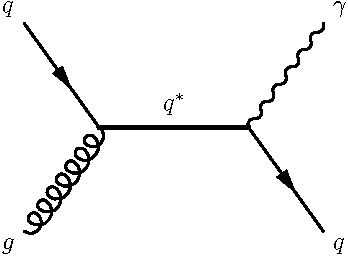
\includegraphics[width=0.3\linewidth]{2_theory/diagrams/qstar_gammajet_s_channel}
    \hspace{1cm}
    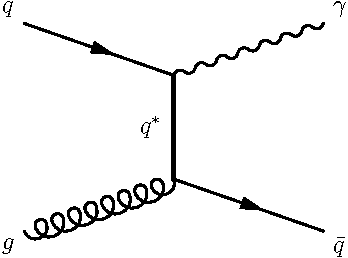
\includegraphics[width=0.3\linewidth]{2_theory/diagrams/qstar_gammajet_t_channel}
    \caption{Feynman diagrams of the \ac{EQ} production in \pp collisions and decay into a quark and a photon in the \(s\)-channel (left) and \(t\)-channel (right).}
    \label{fig:theory:bsm:diagrams}
\end{figure}


In the \ac{SM} there is not a resonance production process decaying into a photon+jet pair in \pp collisions, and direct photon+jet production at tree level occurs via Compton scattering or \qqbar annihilation, as described in \Sect{\ref{subsec:theory:sm:prompt_photon}}. As a result, the \gammajet invariant mass (\myj) distribution is rapidly falling; thus, the \gammajet production mediated by a heavy \ac{EQ} may be discovered if it exists. Hereinafter, in the context of this thesis, \ac{EQ} models are only studied with \gammajet decays. In \fixme{GIVE REFENRECE TO CHAPTER WITH SIGNALS}, information regarding cross sections and the signals signatures in the \ac{ATLAS} detector is given.

\subsection{Higher dimensional theories}

There are at least two seemingly fundamental energy scales in nature, the electroweak scale \(m_{W}~\sim 10^3~\gev\) and the Planck scale \(m_P = G^{-1/2} \sim 10^{18}~\gev\), where \(G\) is the Gravitational constant. Explaining the enormity of the ratio \(m_P / m_W\) has been the prime motivation for constructing extensions of the \ac{SM} such as models with technicolor or low-energy supersymmetry. It is remarkable that these rich theoretical structures have been built on the assumption of the existence of two very disparate fundamental energy scales. However, there is an important difference between these scales. While electroweak interactions have been probed at distances approaching \(\sim m_W^{-1}\), gravitational forces have not remotely been probed at distances \(\sim m_P^{-1}\).

Proposals for a spacetime with more than three spatial dimensions date back to the 1920s, mainly through the work of Kaluza and Klein, in an attempt to unify the forces of nature~\cite{Bailin_Love-1987}. Although their initial idea failed, the formalism that they and others developed is still useful nowadays. Around 1980, string theory proposed again to enlarge the number of space dimensions, this time as a requirement for describing a consistent theory of quantum gravity. The extra dimensions were supposed to be compactified at a scale close to the Planck scale, and thus not testable experimentally in the near future.

A different approach was given by Arkani-Hamed, Dimopoulos, and Dvali (ADD)~\cite{ADD-1998}, where they showed that the weakness of gravity could be explained by postulating two or more flat extra dimensions in which only gravity could propagate. The size of these extra dimensions should range between roughly a millimeter and \(\sim 1/\tev\), leading to possible observable consequences in current and future experiments. Another approach, by Randall and Sundrum (RS)~\cite{RS1-1999_1,RS1-1999_2}, postulates a five-dimensional Anti-deSitter (AdS) spacetime with warped geometry, where the compactification is of the scale of \(1/\tev\).


These low-scale gravity models~\cite{Antoniadis_Arkani_Dimopoulos_Dvali-1998,ADD-1998,RS1-1999_1,RS1-1999_2,Dvali-2008,Dvali-2010} allow for the production of small black holes (\acp{QBH}) in particle collisions~\cite{Argyres-1998,Banks-1999,Giddings-2002}.
\acp{QBH}, unlike semiclassical ones, show significant differences as their mass approaches the Planck scale. Semiclassical black holes decay thermally, losing mass at the Hawking temperature with minimal effect on the surrounding spacetime. However, as the black hole's mass decreases and nears the Planck scale, the influence of back-reaction on the spacetime becomes substantial, and the black hole can no longer maintain thermal equilibrium with its radiation. Microcanonical corrections help refine the decay model, but eventually quantum mechanical effects dominate. When the black hole's Compton wavelength surpasses its Schwarzschild radius, quantum behavior begins to emerge, potentially giving the black hole particle-like properties. At this point, the concepts of a well-defined temperature and entropy break down, making it unlikely that these black holes will decay thermally~\cite{Meade-2008,Alberghi-2006,Alberghi-2007}.

Focusing on black holes with mass slightly above the Planck scale, it's expected that \ac{QBH} decays will not follow a thermal pattern. Instead, decays into only a few particles will likely dominate, and these processes will take place in a small region of spacetime. The \ac{QBH} might behave like a strongly coupled resonance or a gravitationally bound state. After the black hole decays, the \ac{QCD} hadronization process will take place, given the involvement of color charges.

In \pp collisions, only a fraction of the total center of mass energy \sqs is avaiable in the hard-scattering process. By defining \(sx_ax_b \equiv s \tau \equiv \hat{s}\), where \(x_a\) and \(x_b\) are the fractional energies of the two colliding partons (see \Sect{\ref{subsec:theory:sm:hadron_interactions}}), the full cross section \(\sigma\) reads~\cite{Gingrich_Undseth-2020}:
\begin{equation*}
    \sigma_{\pp \to \text{BH} + X}(s) =
    \sum_{a,b}
        \int_{m^2/s}^{1} \dd{\tau}
            \int_{\tau}^{1}
            \frac{\dd{x}}{x}
            f_a\left(\frac{\tau}{x}\right)
            f_b(x)
            \Theta\left(m - m_{\text{th}}\right)
            \hat{\sigma}_{ab\to \text{BH}} (\hat{s} = m^2),
\end{equation*}
where \(a\) and \(b\) go through all the partons, and \(f_a\) and \(f_b\) are the \acp{PDF1} of them. The Heaviside step function \(\Theta\) marks the minimum mass threshold \(m_{\text{th}}\) at which \acp{QBH} could be produced.
The threshold is typically taken to be the Planck scale \(m_P\) for \acp{QBH}, or a few times \(m_P\) for classical black holes. For \acp{QBH} the overall range in which they are considerd to be produced is \(m_P \leq m \leq 3m_P\)~\cite{Gingrich-2010}.
The parton-level cross section \(\hat{\sigma}\) is most often taken to be the geometrical cross-section \(\sigma \sim \pi r_g^2\) with
\begin{equation*}
    r_g = k(D) \frac{1}{m_P} \left(\frac{m}{m_P}\right)^{\frac{1}{D-3}},
\end{equation*}
where \(k(D)\) is a numerical coefficient depending only on the number of dimensions and the definition of the fundamental Planck scale:
\begin{equation*}
    k(D) = 
    \left(
        2^{D-4}
        \left(\sqrt{\pi}\right)^{D-7}
        \frac{\Gamma \left(\frac{D-1}{2}\right)}{D-2}
    \right)
    ^{\frac{1}{D-3}}
\end{equation*}

Based on current experimental and phenomenological limits on the Planck scale, it is unlikely that semiclassical black holes will be accessible at energies produced by the \ac{LHC}. However, if the Planck scale is low enough, \acp{QBH} may be produced in abundance at the \ac{LHC}, and these would appear as resonances in the invariant mass of the final state particles. Concerning only the \gammajet final state, there are six non-thermal black hole states:
\begin{alignat*}{2}
    u + g       & \to QBH^{2/3}     && \to u + \gamma\\
    \bar{d} + g & \to QBH^{1/3}     && \to \bar{d} + \gamma\\
    q + \bar{q} & \to QBH^{0}       && \to g + \gamma\\
    q + g       & \to QBH^{0}       && \to g + \gamma\\
    d + g       & \to QBH^{-1/3}    && \to d + \gamma\\
    \bar{u} + g & \to QBH^{-2/3}    && \to \bar{u} + \gamma,
\end{alignat*}
where \(u\) represents all up-type quarks, \(d\) all down-type quarks and \(q\) all quark flavours. Similarly as the \ac{EQ} model, a more detailed phenomenological description of the models is given in \fixme{GIVE REFENRECE TO CHAPTER WITH SIGNALS}.












\section{\acf{MC} simulations}
\label{sec:theory:mc_simulation}


The \ac{MC} technique is a way of calculating difficult integrals that may be hard to solve by ordinary numerical interpolation methods. High-energy collisions between elementary particles normally produce complex final states, which are populated by many hadrons, leptons, photons and neutrinos. The relation between the final states and the underlying physics description is not simple due to the lack of understanding of the physics and the fact that any analytical approach is not feasible due to the large particle multiplicities. An additional difficulty is related to the need to simulate complicated geometrical factors that represent detectors, a routine situation for experimenters.
\ac{MC} methods allow the generation of complete events with final particles (i.e. hadrons, leptons and photons) together with their momenta, with the same average behaviour and the same fluctuations as the data. Whereas in the data the fluctuations arise from the quantum mechanical character of the underlying theory, in generators these fluctuations are the result of the (quasi-)randomness of the \ac{MC} approach.

The main aspects of the simulated events are: Hard process, Parton Shower, Hadronisation and \acp{UE}, and it follows the schematic representation shown in \Fig{\ref{fig:theory:sm:hadron_interactions:parton_shower}}
The main \ac{MC} event generators used in this thesis are \PYTHIA 8.1~\cite{Pythia8.1}, \PYTHIA 8.2~\cite{Pythia8.2}, \PYTHIA 8.3~\cite{Pythia8.3} and \SHERPA 2.2.2~\cite{Sherpa2.2}.

\subsection{Hard interactions and parton shower}

In order to describe a \(2 \to n\) process from the Lagrangian of the theory (where \(n\) represents a given number of partons in the final state), Feynman diagrams are drawn and evaluated using their specific rules in order to compute the \acp{ME1} in powers of \(\alpha_s\). As the number of partons in the final state increases, the number of Feynman diagrams grows factorially, making higher-order calculations challenging. However, complex processes can be simplified by factoring them into core \(2 \to 2\) processes, which are convoluted with parton splitting probabilities to approximate higher-order effects. Simulation programs implementing this approach are for instance \pythia and \Herwig. These use \ac{LO} perturbative calculations of matrix elements of \(2 \to 2\) processes and implement higher-order \ac{QCD} processes approximately via the so-called initial- and final-state \acp{PS}~\cite{Sjostrand-2006,Dobbs-2004} to produce the equivalent of multi-parton final states.

In a hard process with virtuality \(Q^2\), incoming and outgoing partons emit gluons in a pattern where emissions diverge when gluons become collinear with quarks or when their energy vanishes. Gluon branchings (\(g \to gg\)) exhibit similar divergences, while \(g \to \qqbar\) does not. \ac{NLO} \ac{QCD} programs, such as \Sherpa and \POWHEG, must match \acp{PS} to the \ac{ME1} calculation to avoid double-counting emissions. These emissions, ordered by increasing virtuality, continue until they match the hard process's \(Q^2\). \ac{FSR} similarly decreases parton virtuality until a lower cut-off (\(Q^2_0 \equiv \Lambda_{\text{QCD}} \sim 1~\gev\)) is reached, beyond which perturbation theory loses relevance, and hadronization takes over.

\subsection{Hadronisation}
\label{subsec:theory:mc_simulation:hadronisation}

As the evolution reaches \(Q^2_0 = \Lambda_{\text{QCD}} \), the \ac{PS} phase is truncated since the coupling forces become significant and confinement takes place. This phenomenon cannot still be described from first principles, and therefore, it involves some modelling to transform all the outgoing coloured partons into colourless hadrons of a typical 1 GeV mass scale. The dynamics of this evolution is generally absorbed in fragmentation functions that represents the probability of a parton to fragment into a certain hadron of the final state. Many of these primary hadrons are unstable and decay further at various timescales. Those that are sufficiently long-lived have their decays visible in the detector, or they are stable. There are several models of the hadronisation process, that attempt to connect the results of the \ac{PS} and the final particle spectrum observed. These models can be complemented and tuned using experimental observations. The hadronisation is commonly described by either the Lund string fragmentation model~\cite{Anderson-1983} (as implemented in \Pythia), or the cluster fragmentation model~\cite{Webber-1984} (as implemented in \Herwig and \Sherpa). Essentially, the Lund string fragmentation model asummes a linear confinement, where the energy stored in the colour field between quarks and antiquarks is assumed to increase linearly with the separation of colour charges. Thus, it depicts the colour force by means of a linearly rising potential as charges separate. The potential energy stored increases as partons recede, so it may break up by the production of new quark-antiquark pairs that screen the endpoint colours. Then, quarks and antiquarks may combine to produce hadrons. The cluster fragmentation model is based on the colour preconfinement property of the branching processes, which assumes that the separation of the colour charges forming a singlet are inhibited. After the perturbative parton branching process, the remaining gluons are splitted into light \qqbar pairs, and then neighbouring quarks and antiquarks can be combined into colour singlets (colourless “clusters”), with masses distributions peaking at low values and asymptotically independent of the hard subprocess scale.


\subsection{\acf{UE}}

In addition to the hard interaction that is generated by the \ac{MC} simulation, it is also necessary to account for the interactions between the incoming proton remnants. This is usually modelled through multiple extra \(2 \to 2\) scattering, occurring at a scale of a few GeV. The modelling of the \ac{UE} is crucial in order to give an accurate reproduction of the energy flow that accompanies hard scatterings in hadron colliders. The \ac{UE} can include additional hard interactions and soft processes which can not be calculated perturbatively. These are modelled with adjustable parameters which are tuned to experimental data.



\subsection{Tunes}

Due to the non-perturbative, and therefore incalculable, nature of much of the soft physics processes, like the shower approximations, hadronisation and \ac{UE}, \ac{MC} generators inevitably contain a number of free parameters. These different parameters are usually tuned with data from colliders. A specific set of chosen parameters for a \ac{MC} generator is referred to as a “tune”.
In general, the \ac{ATLAS} \Pythia A14 tune~\cite{Pythia-A14Tune} is used throughout this thesis.
The A14 tune is based on the MONASH tune~\cite{MonashTune} of the \Pythia authors which uses \ee collision data for the hadronisation parameters, and minimum bias \pp collision data at \ac{LHC} to constrain parameters sensitive to initial state radiation and the \ac{UE}. The A14 tune uses in addition a large variety of \ac{ATLAS} data sensitive to multiple parton interactions and \ac{ISR}/\ac{FSR}, and includes jets built from tracks and variables sensitive to the internal jet structure.


\subsection{\acs{ATLAS} detector simulation}

To directly compare the data collected with the \ac{ATLAS} detector with the prediction of \ac{SM} and \ac{BSM} events in simulation, the interaction of the produced particles with the detector material has to be simulated.
The \GEANT~\cite{Geant4} software package is used to simulate the interaction of particles produced in \pp collisions with the different parts of the detector (the \ac{ATLAS} detector is described in \Ch{\ref{ch:atlas}}). \GEANT is an extensive particle simulation package that governs all aspects of the propagation of particles through detectors, based on a description of the geometry of the detector components and the magnetic field. The physics processes include, among others, ionisation, Bremsstrahlung, photon conversions, multiple scattering, scintillation, absorption and transition radiation. The last step involves the digitalisation, which simulates the detector outputs in the same format as the actual raw data. Due to the detailed and complicated geometry of \ac{ATLAS} and the diversity and complexity of the physics processes involved, the consumed computing time per event is large (\(\mathcal{O}\)(1 hour)).

The simulation of a large number of interactions necessary to mimick the \ac{ATLAS} reconstruction is computationally extensive. Especially the simulation of shower developments in the calorimeters consumes a large amount of CPU and computing time. For many \ac{BSM} searches, a large number of parameters affecting the predicted particle masses and interactions have to be simulated, therefore, a "fast" parameterised detector simulation has been developed to cope with this high simulation demand.

A so-called AtlFast3 or AF3~\cite{ATLAS-AF3} (built upon AltFast2~\cite{ATLAS-AF2}) setup simulation chain uses \GEANT~\cite{Geant4} simulation for the interactions in the \ac{ID} and \ac{MS} (described in \Ch{\ref{ch:atlas}}), and two parametrised simulations of the \ac{ECAL} and \ac{HCAL} are used: FastCaloSim V2\footnote{The previous version of AtlFast, called AtlFast2 used FastCaloSim~\cite{ATLAS-FastCaloSim} to simulate the pasage of particles through the calorimeters.}, and FastCaloGAN.
Parametric simulations of the calorimeter response simulate the energy of a particle shower as a single step based on an underlying parametrization instead of simulating how every particle propagates and interacts inside the calorimeter volume.

AtlFast3 introduces several key improvements compared to AtlFast2. Specifically, AtlFast3 enhances the handling of calorimeter showers, significantly improving how energy deposits in the detector cells are simulated. These improvements address limitations in AtlFast2, where sub-cluster structures and lateral shower shapes were not fully described. This new generation also integrates enhanced parameterised simulations and a more precise calorimeter model, leading to improved reconstruction of physics objects like jets and missing transverse energy. These changes lead to better agreement between fast simulation and full simulation results.
Moreover, AtlFast3 supports more advanced algorithms for tracking and calorimeter simulation, ensuring that discrepancies seen in AtlFast2 are minimized, such as inaccuracies in shower shapes and fluctuations.

